\PassOptionsToPackage{xetex,dvipsnames}{xcolor}
\PassOptionsToPackage{xetex}{graphicx}
\documentclass[xetex]{beamer}
% ---- Minimal setup (XeLaTeX) ----
\usepackage{fontspec}
\defaultfontfeatures{Ligatures=TeX}
%\usepackage{luatexja}
%\usepackage{luatexja-fontspec}
%\ltjsetparameter{jacharrange={-9}}
\setmainfont{TeX Gyre Pagella}
\setsansfont{TeX Gyre Heros}
\setmonofont{Inconsolata} % TeX Gyre Cursor} %  Fira Mono}
% Auto-switch by Unicode block
% Font families for non-Latin scripts
\newfontfamily\jafont{Noto Sans CJK JP}
\newfontfamily\krfont{Noto Sans CJK KR}
\newfontfamily\hanfont{Noto Sans CJK SC}
\newfontfamily\devanagarifont{Noto Sans Devanagari}
\newfontfamily\ipafont{Gentium}

% Explicit font-switching macros — use these to wrap non-Latin text
\newcommand{\ja}[1]{{\jafont #1}}          % Japanese
\newcommand{\cn}[1]{{\hanfont #1}}         % Chinese/Mandarin
\newcommand{\ko}[1]{{\krfont #1}}          % Korean
\newcommand{\dv}[1]{{\devanagarifont #1}}  % Devanagari
\newcommand{\ipa}[1]{{\ipafont #1}}        % IPA
\newcommand{\jpf}[1]{\ja{#1}}             % backward-compat alias

% Graceful fallback in PDF bookmarks
\pdfstringdefDisableCommands{%
  \def\ja#1{#1}%
  \def\cn#1{#1}%
  \def\ko#1{#1}%
  \def\dv#1{#1}%
  \def\ipa#1{#1}%
  \def\jpf#1{#1}%
}
% \newfontfamily\emoji{Noto Color Emoji}[Renderer=Harfbuzz,Scale=MatchLowercase]
% \newcommand{\e}[1]{{\emoji #1}}

\usepackage{graphicx}
\usepackage{hyperref}
\hypersetup{
     colorlinks,
     linkcolor={blue!50!black},
     citecolor={red!50!black},
     urlcolor={blue!80!black}
   }
\usepackage{booktabs}
\usepackage{microtype}

\newcommand{\txx}[1]{\textbf{\textcolor{blue}{#1}}}

% --- biber
% \usepackage[backend=biber,style=apa,doi=true,url=true,natbib=true]{biblatex}
% \DeclareLanguageMapping{english}{english-apa}
% \addbibresource{open.bib}
\usepackage[round]{natbib}

% ---- Beamer look ----
\usetheme{Boadilla}
\usecolortheme{seahorse}
\setbeamertemplate{navigation symbols}{}
\setbeamertemplate{itemize items}[circle]
\setbeamertemplate{itemize subitem}[triangle]
%\setbeamertemplate{footline}[frame number]
\setbeamerfont{block body example}{size=\small}
\setbeamerfont{block title example}{size=\small}  % optional: adjust title too
% ---- Section outline slide ----
\AtBeginSection[]{
  \begin{frame}
    \frametitle{Roadmap}
    \small
    \tableofcontents[currentsection, hideothersubsections]%, hideallsubsections]
  \end{frame}
}
\logo{
\includegraphics[width=15mm]{img/UP_logo_FF_horizont_en.png}}

% ---- other packages
\usepackage{tikz}

% ---- Linguistics

\usepackage{langsci-gb4e}
\usepackage{avm}

\usepackage[normalem]{ulem}
\newcommand{\ul}{\uline}
\newcommand{\ull}{\uuline}
\newcommand{\udl}{\dashuline}
\newcommand{\uwl}{\uwave}

\usepackage[e,f,j]{mtg2e}
\newcommand{\cmn}{\mtciteform}
\newcommand{\kor}{\mtciteform}
\renewcommand{\mtcitestyle}[1]{\textcolor{teal}{\textit{#1}}}
\usepackage{xcolor}
 \newcommand{\bs}{\textbackslash}   % backslash
 \newcommand{\cmd}[1]{{\bf \color{red}#1}}   % highlights command
 \newcommand{\wemp}[1]{\ul{#1}}   % highlight
 \newcommand{\emp}[1]{\textbf{\color{blue}{#1}}}   % highlight
 \newcommand{\rel}[1]{\textsc{\color{blue}{#1}}}
 %%% imi zokusei
 \newcommand{\iz}[1]{\textup{\texttt{\color{blue}{\textbf{#1}}}}}
 \newcommand{\con}{\iz}
 \newcommand{\lnk}[1]{\rel{#1}}
 \newcommand{\dff}[1]{\rel{#1}}
\newcommand{\cmp}[1]{{[\textsc{#1}]}}
\newcommand{\elem}[1]{\ensuremath{\langle}\texttt{#1}\ensuremath{\rangle}}
 \newcommand{\lex}[1]{\textbf{\color{teal}{\textit{#1}}}}
 \newcommand{\lng}[1]{\textcolor{teal}{\textit{#1}}}
\newcommand{\wn}[3]{\lex{#1}\ensuremath{_{#2:#3}}}
\usepackage{relsize,xspace}
\newcommand{\wnida}[1]{\asort{\wnid{#1}}}
\newcommand{\wnid}[1]{\textsf{\smaller #1}}
\newcommand{\topic}[1]{\textsc{#1}}
\newcommand{\into}{\ensuremath{\rightarrow}\xspace}
\newcommand{\ent}{\ensuremath{\Rightarrow}\xspace}
\newcommand{\nent}{\ensuremath{\not\Rightarrow}\xspace}
\newcommand{\tot}{\ensuremath{\leftrightarrow}\xspace}

\newcommand{\MyLogo}[1]{}

% \newcommand{\task}{\marginpar{\raisebox{-2ex}{
%       \hspace{-0.5em}\reflectbox{\includegraphics[width=2em]{img/detective.pdf}}}}}
\newcommand{\task}{?}


\setbeamercolor{taskc}{fg=black,bg=red!10}

\newenvironment{taskb}[1][]{%
  \begin{beamercolorbox}[rounded=true,shadow=true,wd=\linewidth,sep=0.5em]{taskc}
    \ifx\relax#1\relax
      % No title - just show content
    \else
      % Title provided
      \textbf{\large ?} #1
      \par\vspace{0.3em}
    \fi
}{%
  \end{beamercolorbox}
  \vspace{0.5em}
}

\title[Wordnets and Metaphor]{Multilingual Modelling with Wordnets:
  \\ Metonymy Travels, Metaphor Wanders}
%\\[2ex] \bl{Picking Brains, Crossing Ideas}}
\author[Bond and many more]{Francis \textbf{Bond} 
  \\ and many, many more}
\institute[Palacký]{General Linguistics and Asian Studies,
\\  Palacký University, Olomouc, Czechia
\\[1.5ex] \url{<bond@ieee.org>}}

\date[2026]{University of Ljubljana, April 2026}
\newcommand{\ili}[1]{\href{http://www.globalwordnet.org/ili/#1}{\url{#1}}}

%%% make it smaller
 % gs -sDEVICE=pdfwrite -dCompatibilityLevel=1.4 -dPDFSETTINGS=/printer -dNOPAUSE -dQUIET -dBATCH -sOutputFile=omw-teanga-small.pdf omw-teanga.pdf 
\usepackage{chainnet}
\usepackage{booktabs}
\newcommand{\clex}[1]{\textbf{\texttt{#1}}}
\newcommand{\ldiff}[1]{\textbf{\texttt{#1}}}
\newcommand{\dom}[1]{\textbf{\texttt{#1}}}

\newcommand{\LEX}[6][]{\textbf{\textit{#2}} \textit{#1} (#3: #4) #5 --- \textit{#6}}

\usepackage{tcolorbox}
% Define your custom style
\tcbset{
    lightbox/.style={
        boxsep=2pt,
        colback=blue!5!white,
        colframe=gray!20,
        boxrule=0.2pt,
        width=0.3\textwidth
    }
}\tcbset{
    fullbox/.style={
        boxsep=2pt,
        colback=blue!5!white,
        colframe=gray!20,
        boxrule=0.2pt,
        width=\textwidth
    }
}
\newcommand{\onew}[1]{\hspace*{-0.5em}\colorbox{black!20}{#1}}

\newcommand{\wns}[2]{\textit{\textbf{#1}}\,\ensuremath{_#2}}

%\usepackage[hidelinks]{hyperref}
\hypersetup{ 
     colorlinks, 
     linkcolor={blue!50!black},
     citecolor={red!50!black},
     urlcolor={blue!80!black}
}


\usepackage{array}
\newcolumntype{H}{>{\setbox0=\hbox\bgroup}c<{\egroup}@{}}

\usepackage[round]{natbib}
\usepackage{fontenc}
\usepackage{polyglossia}
\setmainlanguage{english}
\usepackage{xeCJK}
%\setCJKmainfont{WenQuanYi Micro Hei}
% \setmainfont[Numbers=OldStyle]{TeX Gyre Pagella}
%\setCJKmainfont{Droid Sans Fallback}
\setCJKmainfont{Noto Sans CJK SC}
\usefonttheme{professionalfonts}
\setsansfont{Linux Libertine O}

 \usepackage{qtree,avm,expex}
\definelingstyle{cmn}{everygla=,
everyglb=\itshape,everyglc=\footnotesize}

\usepackage{relsize,xspace}


\usetheme{Boadilla}
\usecolortheme{seahorse}
\setbeamertemplate{navigation symbols}{}
% ---- Section outline slide ----
\AtBeginSection[]{
  \begin{frame}
    \frametitle{Roadmap}
    \small
    \tableofcontents[currentsection, hideothersubsections]%, hideallsubsections]
  \end{frame}
}
\logo{
\includegraphics[width=15mm]{img/UP_logo_FF_horizont_en.png}}

\newcommand{\zhong}{\ensuremath{[\Big|]}}
% NUS Meeting Room 1 (MR 1) 	COM1-03-19
\newcommand{\bl}[1]{\textcolor{blue}{#1}}
%\newcommand{\sh}[1]{\textcolor{blue}{#1}}
\newcommand{\txx}[1]{\textbf{\textcolor{blue}{#1}}}
\usepackage{url}

%\newcommand{\wn}{\url}
\usepackage[e,f,j]{mtg2e}
\newcommand{\cmn}{\mtciteform}
\newcommand{\kor}{\mtciteform}
\renewcommand{\mtcitestyle}[1]{\textcolor{teal}{\textit{#1}}}
\usepackage{xcolor}
 \newcommand{\bs}{\textbackslash}   % backslash
 \newcommand{\cmd}[1]{{\bf \color{red}#1}}   % highlights command
 \newcommand{\wemp}[1]{\ul{#1}}   % highlight
 \newcommand{\emp}[1]{\textbf{\color{blue}{#1}}}   % highlight
 \newcommand{\rel}[1]{\textsc{\color{blue}{#1}}}
 \newcommand{\lnk}[1]{\rel{#1}}
 \newcommand{\dff}[1]{\texttt{\color{blue}{#1}}}

 \newcommand{\lex}[1]{\textbf{\color{teal}{\textit{#1}}}}
 \newcommand{\lng}[1]{\textcolor{teal}{\textit{#1}}}
\newcommand{\wn}[3]{\lex{#1}\ensuremath{_{#2:#3}}}
\usepackage{relsize}
\newcommand{\wnida}[1]{\asort{\wnid{#1}}}
\newcommand{\wnid}[1]{\textsf{\smaller #1}}

\usepackage{mygb4e,url}
\usepackage[normalem]{ulem}
\newcommand{\ul}{\uline}
\newcommand{\ull}{\uuline}
\newcommand{\udl}{\dashuline}
\newcommand{\uwl}{\uwave}

\newcommand{\MyLogo}[1]{(#1)}

\newcommand{\sh}[1]{https://fcbond.github.io/sh-canon/#1.html}
\newcommand{\SCAN}{\href{\sh{scan}}{\textit{A Scandal in Bohemia}}\xspace}
\newcommand{\REDH}{\href{\sh{redh}}{\textit{The Redheaded League}}\xspace}
\newcommand{\HOUN}{\href{\sh{houn}}{\textit{The Hound of the
      Baskervilles}}\xspace}
\newcommand{\SPEC}{\href{\sh{spec}}{\textit{The Adventure of the Speckled Band}}\xspace}
\newcommand{\DANC}{\href{\sh{danc}}{\textit{The Adventure of the Dancing Men}}\xspace}
\newcommand{\FINA}{\href{\sh{fina}}{\textit{The Adventure of the Final Problem}}\xspace}
\newcommand{\NAVA}{\href{\sh{nava}}{\textit{The Adventure of the Naval Treaty}}\xspace}

\newcommand{\swn}{SentiWordNet\xspace}
\newcommand{\plwn}{plWordNet\xspace}
\newcommand{\plemo}{plWordNet~emo\xspace}
\newcommand{\pwn}{Princeton WordNet\xspace} 
\newcommand{\mlsc}{ML-SentiCon\xspace}
\newcommand{\wnop}{\textsc{Micro-WNOp}\xspace}
\newcommand{\ntumc}{NTU-MC\xspace}


\begin{document}
\maketitle
\lingset{lingstyle=cmn}
\begin{frame}{Outline}
   \tableofcontents
 \end{frame}


\section{Metaphor}
\begin{frame}{Metaphor and Metonymy}

  \begin{itemize}
  \item Metaphor and Metonymy are two fundamental tropes (figures of speech)
  \item Both play crucial roles in the way we understand and use language
  \item \txx{Metaphor} involves understanding one concept in terms of
    another, often unrelated, concept.
     \begin{itemize}
    \item \eng{This horse has a \ul{chestnut} on its leg} ``a small horny bump''
    \item Metaphors create new concepts in the target domain by
      mapping elements from the source domain
    \end{itemize}
    \item They are crucial in understanding novel uses of words
  \item \txx{Metonymy} involves the substitution of one term for
    another to which it is closely related
    \begin{itemize}
    \item \eng{I ate a \ul{chestnut}}
    \item \eng{I pruned the \ul{chestnut} [tree]}
    \item \eng{This table is made from \ul{chestnut} [wood]}
    \item Metonymy works by contiguity or association between concepts,
      usually by some shared attribute, or by a part-whole relation
    \end{itemize}
  \end{itemize}

\end{frame}


\begin{frame}{The state-of-the art}

  \begin{itemize}
  \item Conceptual Metaphor research very wide spread (cognitive, computational, therapeutic, political)
    \begin{itemize}
    \item A lot of fantastic research!
    \end{itemize}
  \item No broad coverage multilingual inventory of metaphors
    \begin{itemize}
    \item MetaNet --- long-running but mainly English (some Spanish and Chinese, far from comprehensive)
    \item \href{https://metaphorshare.com/}{MetaphorShare} --- new
      (2025) initiative to bring together resources, but most with only
      hundreds or thousand of examples.
    \end{itemize}
  \item No broad coverage multilingual corpora of instances
    \begin{itemize}
    \item MIPVU is the largest (mainly English, some work in other languages)
    \end{itemize}
  \item No broad coverage multilingual metaphor interpretation tools
    \begin{itemize}
    \item Some tools for identification
    \item Some tools for paraphrasing, but biased toward English (LLMs)
    \end{itemize}
  \end{itemize}
  
\end{frame}


\begin{frame}{SoA: scattered fragments of the metaphor landscape}
  \centering
  
\includegraphics[width=0.95\textwidth]{img/bond_metaphor_diagram_1.png}
%  \caption{The state-of-the-art: scattered fragments of the metaphor landscape}\label{fig:fragment}
\end{frame}

\begin{frame}{We are trying a different approach}
  \begin{itemize}
  \item Exploit existing multilingual resources (wordnets and sense-annotated corpora)
  \item ChainNet links word senses by metaphor --- for all$^*$ nouns in the English wordnet
  \item Use ChainNet to study metaphor over a (quite) complete vocabulary
    \begin{itemize}
    \item Link lexical to conceptual metaphors
    \item Find unknown conceptual metaphors (unlinked lexical metaphors)!
    \item \textbf{Finish with a much more complete understanding}
    \item Use wordnet sense tagged corpora to investigate attested uses
    \item \textbf{Finish with a grounded, quantitative understanding}
    \end{itemize}
  \end{itemize}
\end{frame}




\section{ChainNet}
\label{sec:chainnet}



\begin{frame}{ChainNet}

  \begin{itemize}
  \item ChainNet is an attempt to comprehensively model these tropes \citep{maudslay-etal-2024-chainnet-structured,Bond:Maudslay:2025}
    \begin{itemize}
    \item All nouns (word + synset combinations) in the
      Princeton Wordnet 3.0 \citep{_Fellbaum:1998} with three or more senses$^*$
      were annotated
    \item Every sense linked to another sense, or treated as a homonym (unrelated)
      \begin{itemize}
      \item 7,500 metaphor pairs
      \item 6,116 metonymy pairs
      \end{itemize}
  \item Most annotated by 1 annotator, some by 2 annotators
    \begin{itemize}
    \item Inter-annotator agreement 70\% (88\% for same prototype)
    \item Intra-annotator agreement 81\% (92\% for same prototype)
    \end{itemize}
  \item Originally grew out of work in determining homonyms --- which senses of a word are related
  \end{itemize}

\end{itemize}

\begin{small}
 $^*$ almost, and some with two senses.   All should eventually be annotated \\
\end{small}
\end{frame}
\begin{frame}{chestnut}
    \begin{center}
\begin{tikzpicture}[derivation]

\litbox[4cm]{1}{at (0,0)}{\sense{chestnut}{3} edible nut of any of various chestnut trees}

\assbox[4cm]{3}{[below right = -5mm and 2cm of 1]}{%
\sense{chestnut}{2} any of several attractive deciduous trees yellow-brown in autumn; yield a hard wood and edible nuts in a prickly bur}

\assbox[2cm]{4}{[below right = 0.85cm and -1cm of 1]}%
{\sense{chestnut}{4} the brown color of chestnuts}

\assbox[3cm]{6}{[below  = 8mm of 4]}{\sense{chestnut}{6} a dark golden-brown or reddish-brown horse }

\metbox[3cm]{5}{[below left = 0.8cm and -3cm of 1]}%
{\sense{chestnut}{5} a small horny callus on the inner surface of a horse's leg}

\assbox[4cm]{2}{[below = 13mm  of 3]}{\sense{chestnut}{1}  [\synonym{chestnut tree}] wood of any of various chestnut trees of the genus Castanea }

   \path[related] (1) edge node[anchor=south, font={\footnotesize}] {\relatededgelabel} (3);

%  \node[shape=coordinate] (origin) [above = .8cm of 4, node contents={}];

  \path[related] (3) edge node[anchor=west, font={\footnotesize}] {\relatededgelabel} (2);

    % \node[shape=coordinate] (origin2) [above left = .8cm and -.5cm of 2, node contents={}];
    % \node[shape=coordinate] (origin3) [below = .8cm of origin2, node contents={}];

 % \path[analogy] (origin2) edge node[anchor=west, font={\footnotesize}] {\metaphoricaledgelabel} (origin3);

 \path[analogy] (1) edge node[anchor=south, xshift = -8mm, yshift=-3mm, font={\footnotesize}] {\metaphoricaledgelabel} (5);
 %\node[shape=coordinate] (origin) [above = .4cm of 5, node contents={}];
 
 \path[related] (1) edge node[anchor=south,  xshift = 9mm, yshift=-3mm, font={\footnotesize}] {\relatededgelabel} (4);

 \path[related] (4) edge node[anchor=south,  xshift = 9mm, yshift=-3mm, font={\footnotesize}] {\relatededgelabel} (6);

%  \node[shape=coordinate] (origin) [above = .4cm of 5, node contents={}];

\end{tikzpicture}
\end{center}

\end{frame}



\begin{frame}{Metaphor viewed through the lexicon: a broader view}
  \centering
  
\includegraphics[width=0.9\textwidth]{img/bond_metaphor_diagram_2.png}
%  \caption{Metaphor viewed through the lexicon: a broader view}\label{fig:lexicon}
\end{frame}


\begin{frame}{How we proceed}
\begin{itemize}
\item  For every word with more than two senses
  \begin{itemize}
  \item examine all pairs
  \item determine if they are  linked by metaphor or metonymy, or not at all
  \end{itemize}
  \begin{tcolorbox}
    \wns{darkness}{1} --- absence of light or illumination \hfill (from wordnet)\\
    \wns{darkness}{2} --- an unilluminated area “he moved off into the darkness” \\
    \wns{darkness}{3} --- absence of moral or spiritual values “the powers of darkness” \\
    \wns{darkness}{4} --- an unenlightened state “he was in the dark concerning their intentions” “his lectures dispelled the darkness” \\
    \raisebox{0.5ex}{\rule{\textwidth}{0.4pt}} 
     \wns{darkness}{1} $\rightarrow$  \wns{darkness}{2} (metonymy)\\
     \wns{darkness}{1} $\rightarrow$  \wns{darkness}{3} (metaphor) \\
     \wns{darkness}{1} $\rightarrow$  \wns{darkness}{4} (metaphor)
  \end{tcolorbox}
\end{itemize}
\end{frame}

\begin{frame}{Exploit wordnet for a richer view}
  \begin{itemize}
  \item Once we have senses, we can look at supersenses
    \begin{tcolorbox}
      \wns{darkness}{1} (state) $\rightarrow$  \wns{darkness}{3} (state)  \\
      \wns{darkness}{1} (state) $\rightarrow$  \wns{darkness}{4} (cognition) 
    \end{tcolorbox}
   \item Or indeed any hypernym
    \begin{tcolorbox}
      \wns{darkness}{1} (illumination|state|attribute|TOP) $\rightarrow$  \wns{darkness}{3} (wickedness|condition|sate|attribute|TOP)  \\
      \wns{darkness}{1} (illumination|state|attribute|TOP)) $\rightarrow$  \wns{darkness}{4} (unenlightenment|ignorance|knowledge|\ldots{}|top) 
    \end{tcolorbox}
  \item We will use these to establish Conceptual Metaphor Labels
    \begin{tcolorbox}
      \wns{darkness}{1} $\rightarrow$  \wns{darkness}{3}  = GOODNESS IS LIGHT  \\
      \wns{darkness}{1} $\rightarrow$  \wns{darkness}{4}  =  UNDERSTANDING IS LIGHT
    \end{tcolorbox}
  \end{itemize}
\end{frame}

\begin{frame}{Link to Sense-tagged corpora}
 Finally, we combine this with examples from sense annotated corpora, giving frequencies of metaphorical and non-metaphorical uses.

 \begin{tcolorbox}[title=Examples from \textit{The Adventure of the Speckled Band} (English)]
   \begin{itemize}
   \item \textit{Oh, sir, do you not think that you could help me, too, and at least throw a little light through the dense  \wns{darkness}{4} which surrounds me?}
   \item \textit{``Do you know, Watson,'' said Holmes as we sat together in the gathering \wns{darkness}{1}, ``I have really some scruples as to taking you to-night.}
   \item \textit{Then he turned down the lamp , and we were left in \wns{darkness}{1}.} 
   \end{itemize}
 \end{tcolorbox}

We have at least one story manually annotated for  Bulgarian, English, Mandarin Chinese, Indonesian, Italian, Japanese and Polish, and automatically for Dutch and German. 
 
\end{frame}

\begin{frame}{Metaphor linked to wordnet and corpora: a richer view}
  \centering
  
\includegraphics[width=0.9\textwidth]{img/bond_metaphor_plain.png}
%  \caption{Metaphor viewed through the lexicon linked to corpora: a richer view}\label{fig:corpus}
\end{frame}

\subsection{Some new results}
\begin{frame}{Differences Between Metaphors and Metonyms}
  We can use the wordnet graph to compare the two

  \begin{itemize}
  \item For all trope pairs we measure the path distance between the source and target
  \item We measure the depth in the hierarchy (distance from root)
  \item We measure the number of synonyms of source and target
  \item We also look at the distribution of the topics, \ldots
  \end{itemize}
  \begin{center}
    These are new results (unpublished)
  \end{center}
\end{frame}

\begin{frame}{Path Distance Comparison}
  \begin{center}
    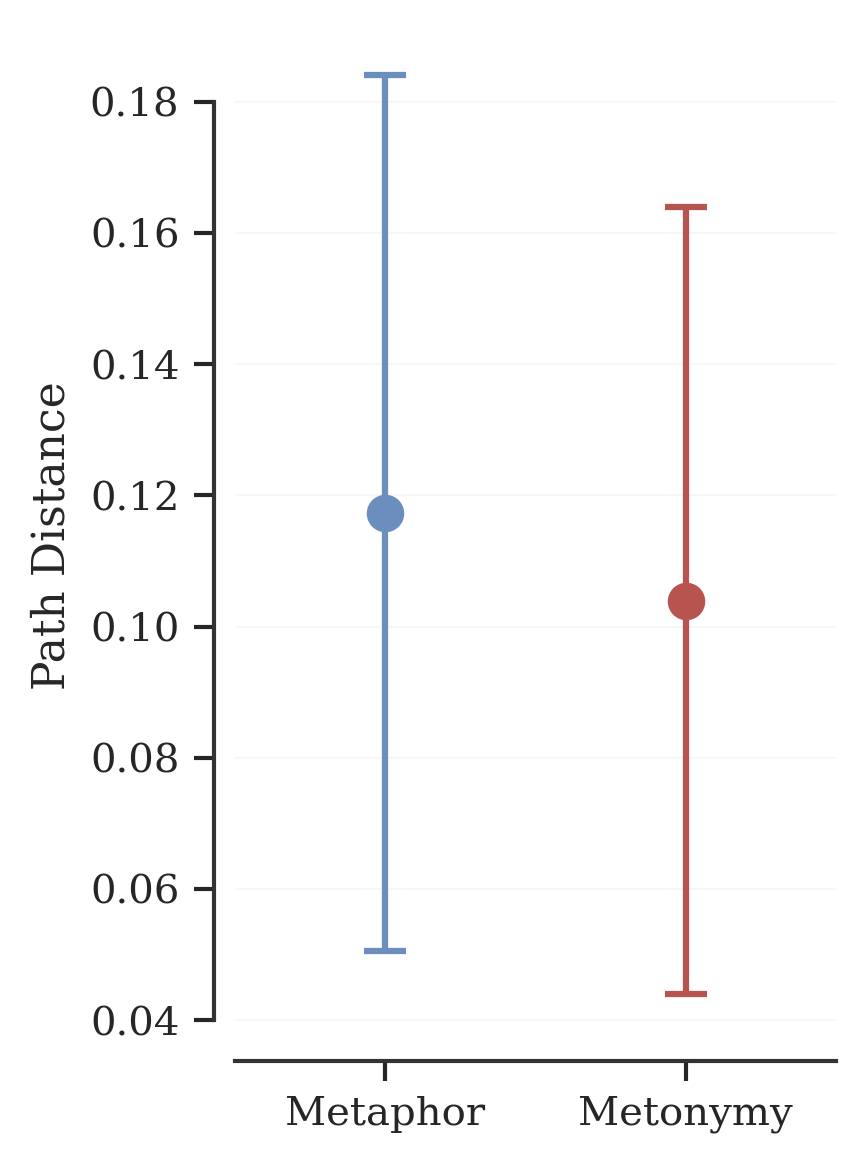
\includegraphics[height=0.9\textheight]{img/path_distance_comparison_errorbar.png}
  \end{center}
\end{frame}
\begin{frame}{Depth in Hierarchy}
  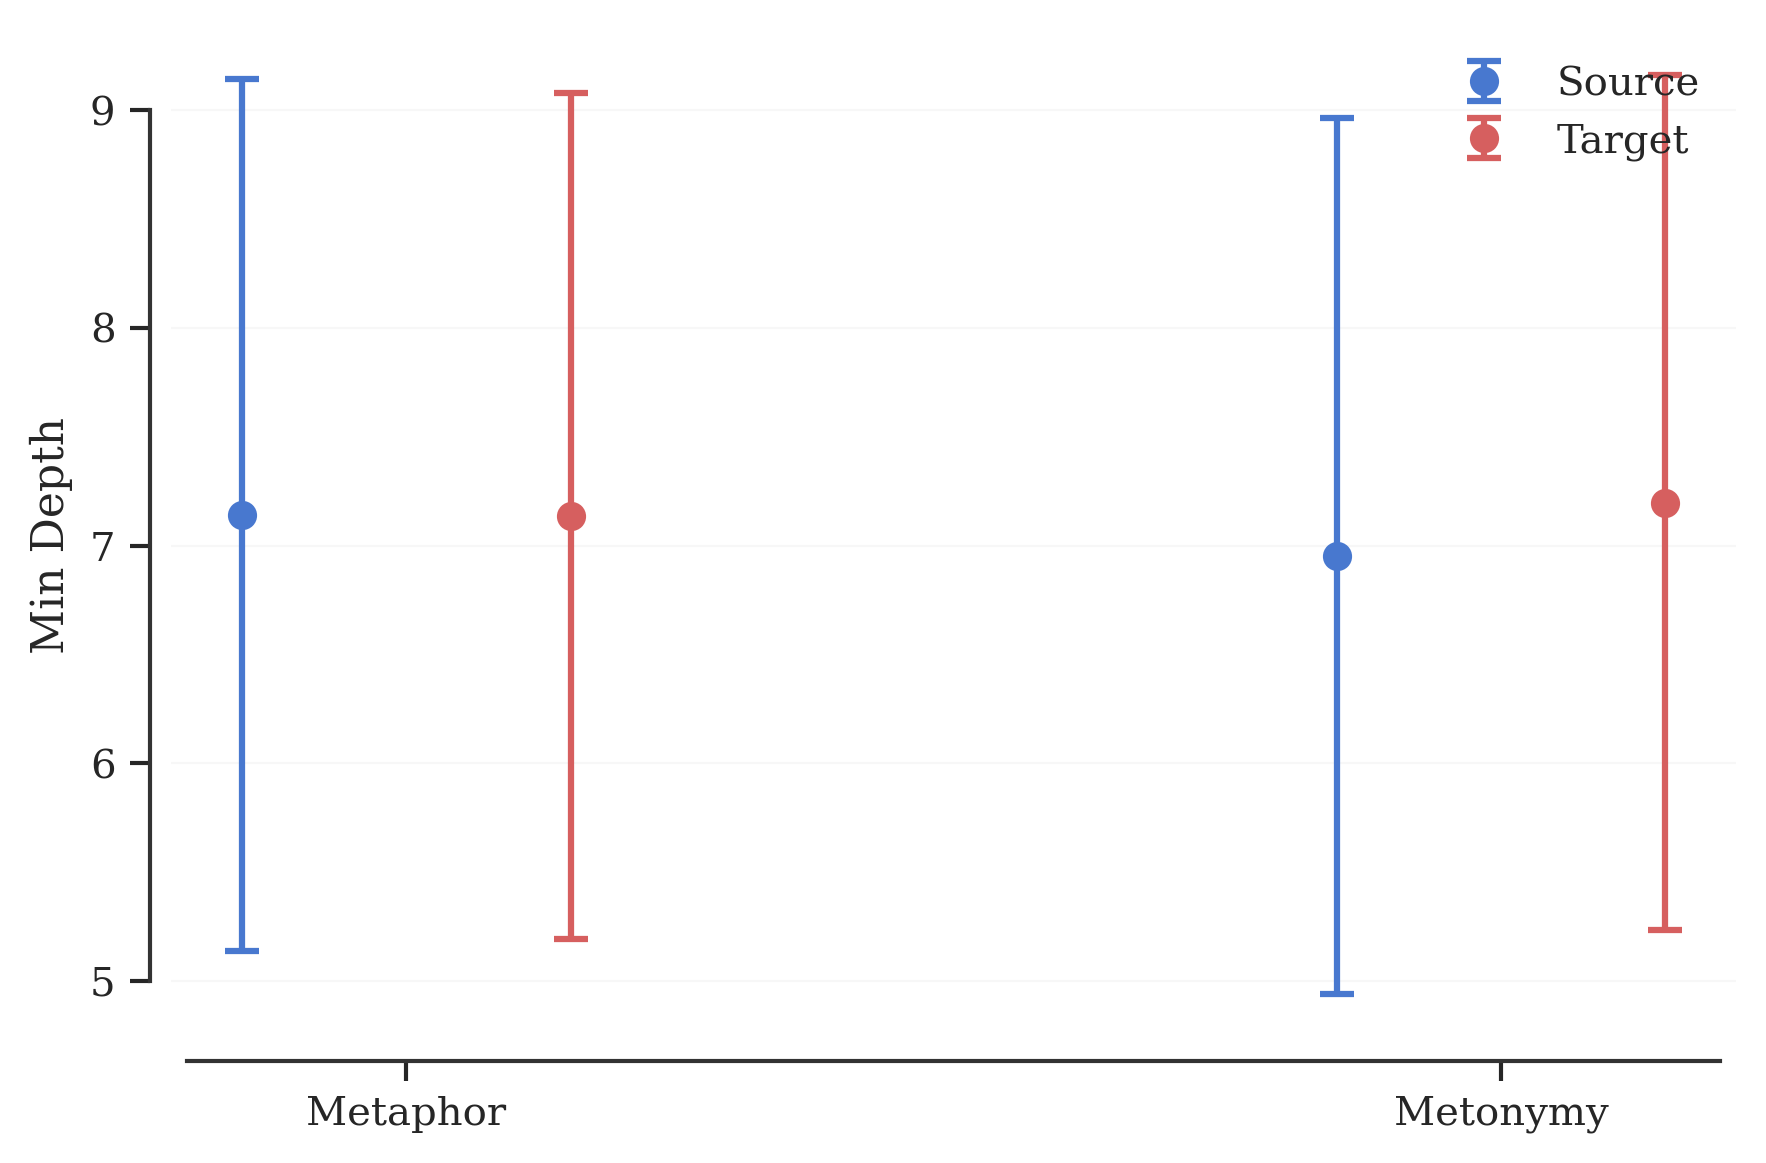
\includegraphics[height=0.9\textheight]{img/depth_comparison_errorbar.png}
\end{frame}
\begin{frame}{Synonymy density (number of synonyms)}
  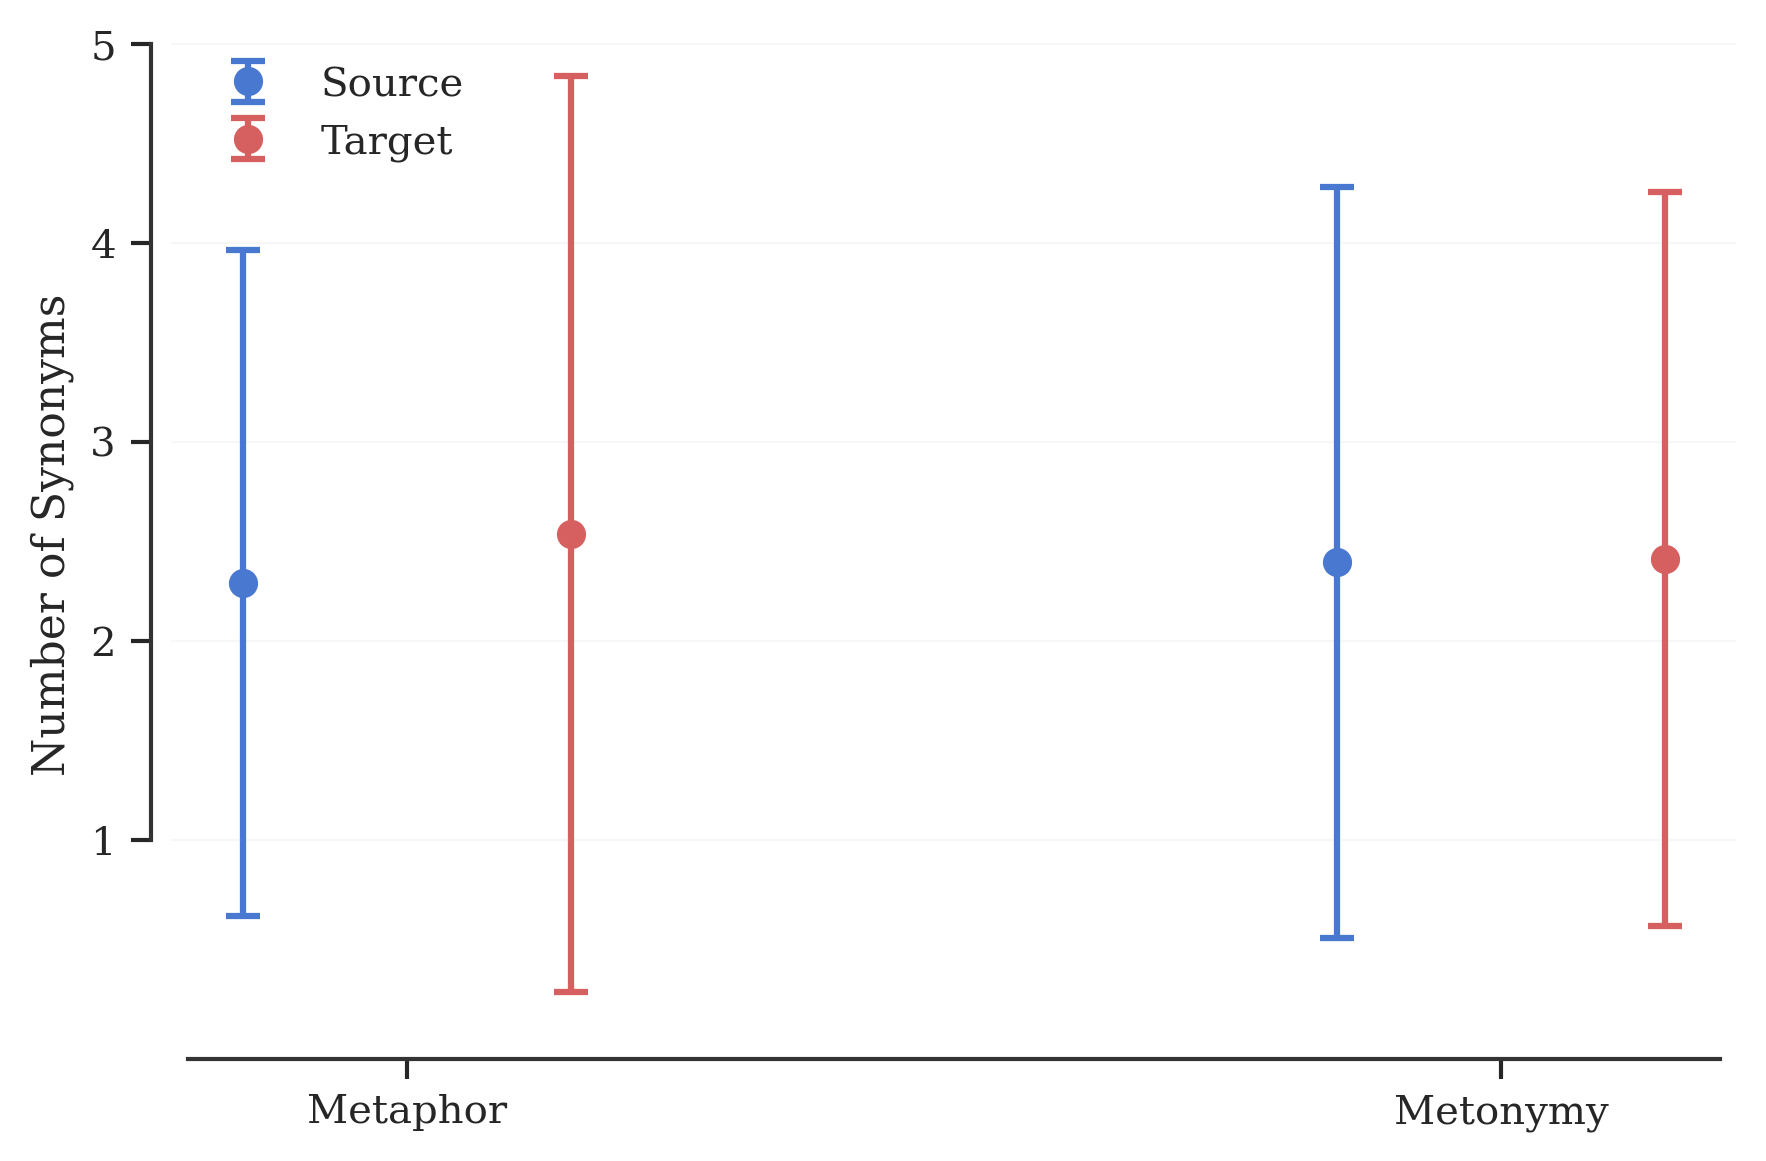
\includegraphics[height=0.9\textheight]{img/synonyms_comparison_errorbar.png}
\end{frame}
\begin{frame}{Topic Heatmap for Metaphors}
  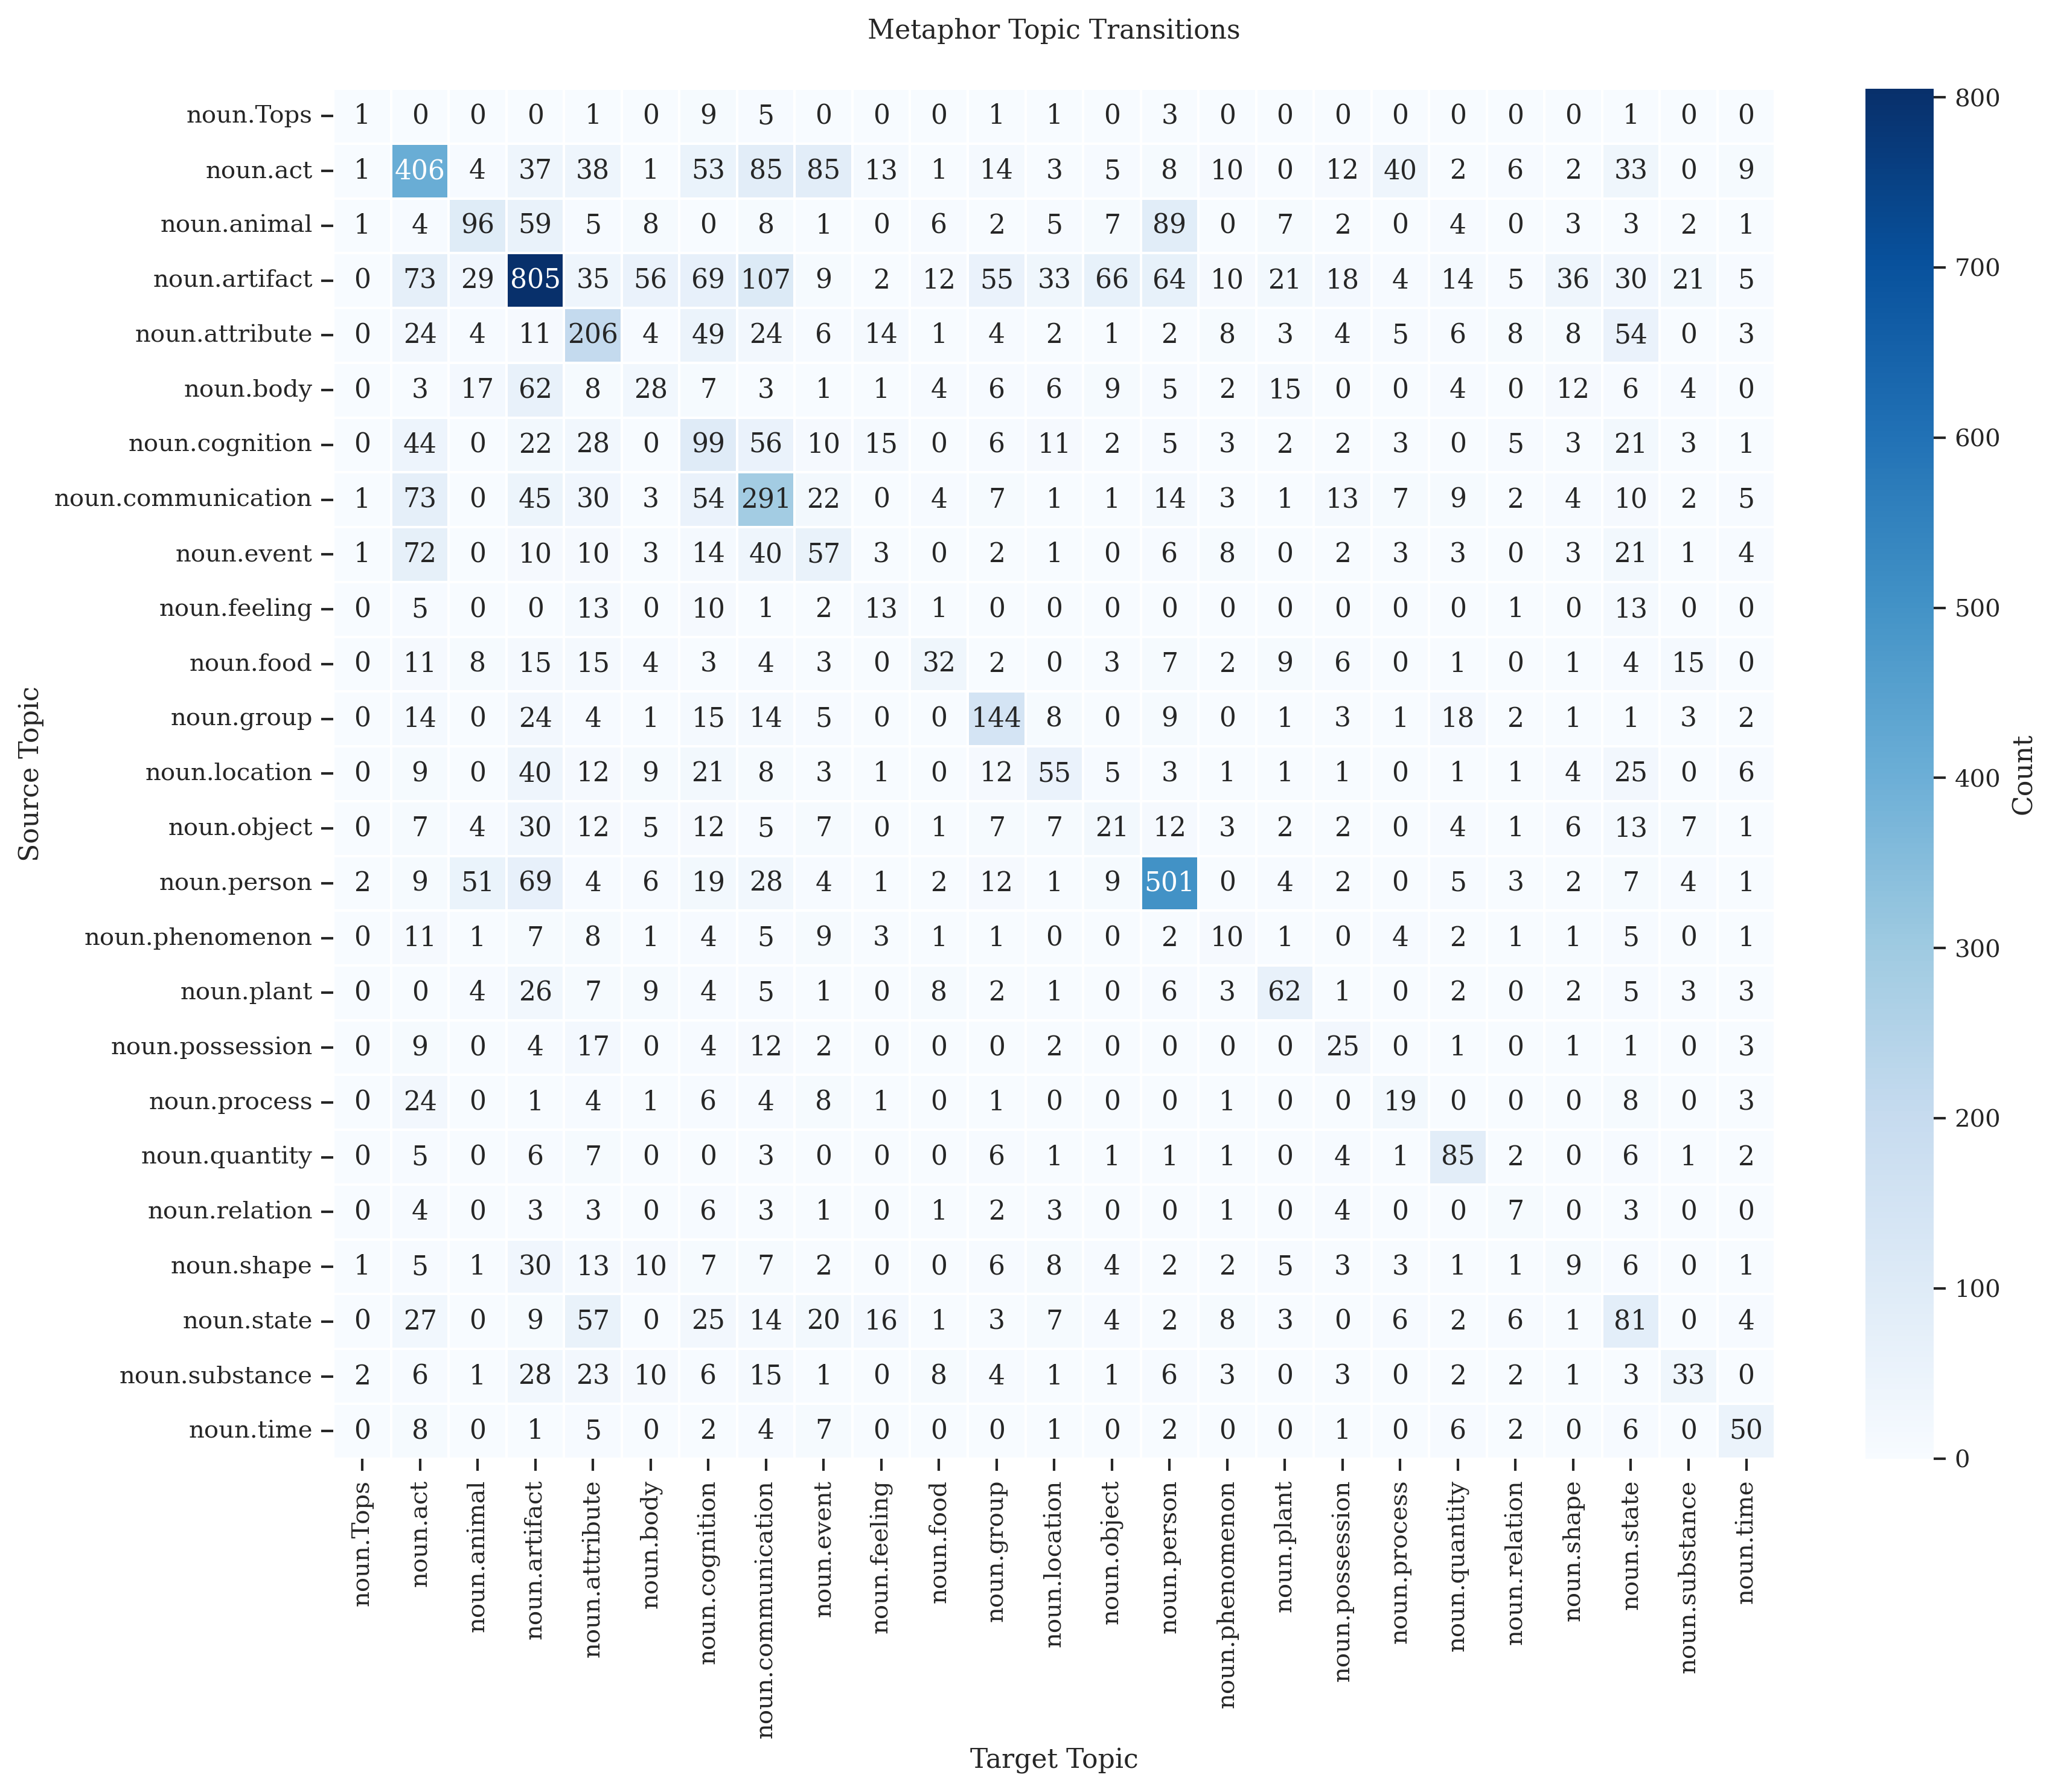
\includegraphics[height=0.9\textheight]{img/metaphor_topic_heatmap.png}
\end{frame}  

\begin{frame}{Topic Heatmap for Metonyms}
 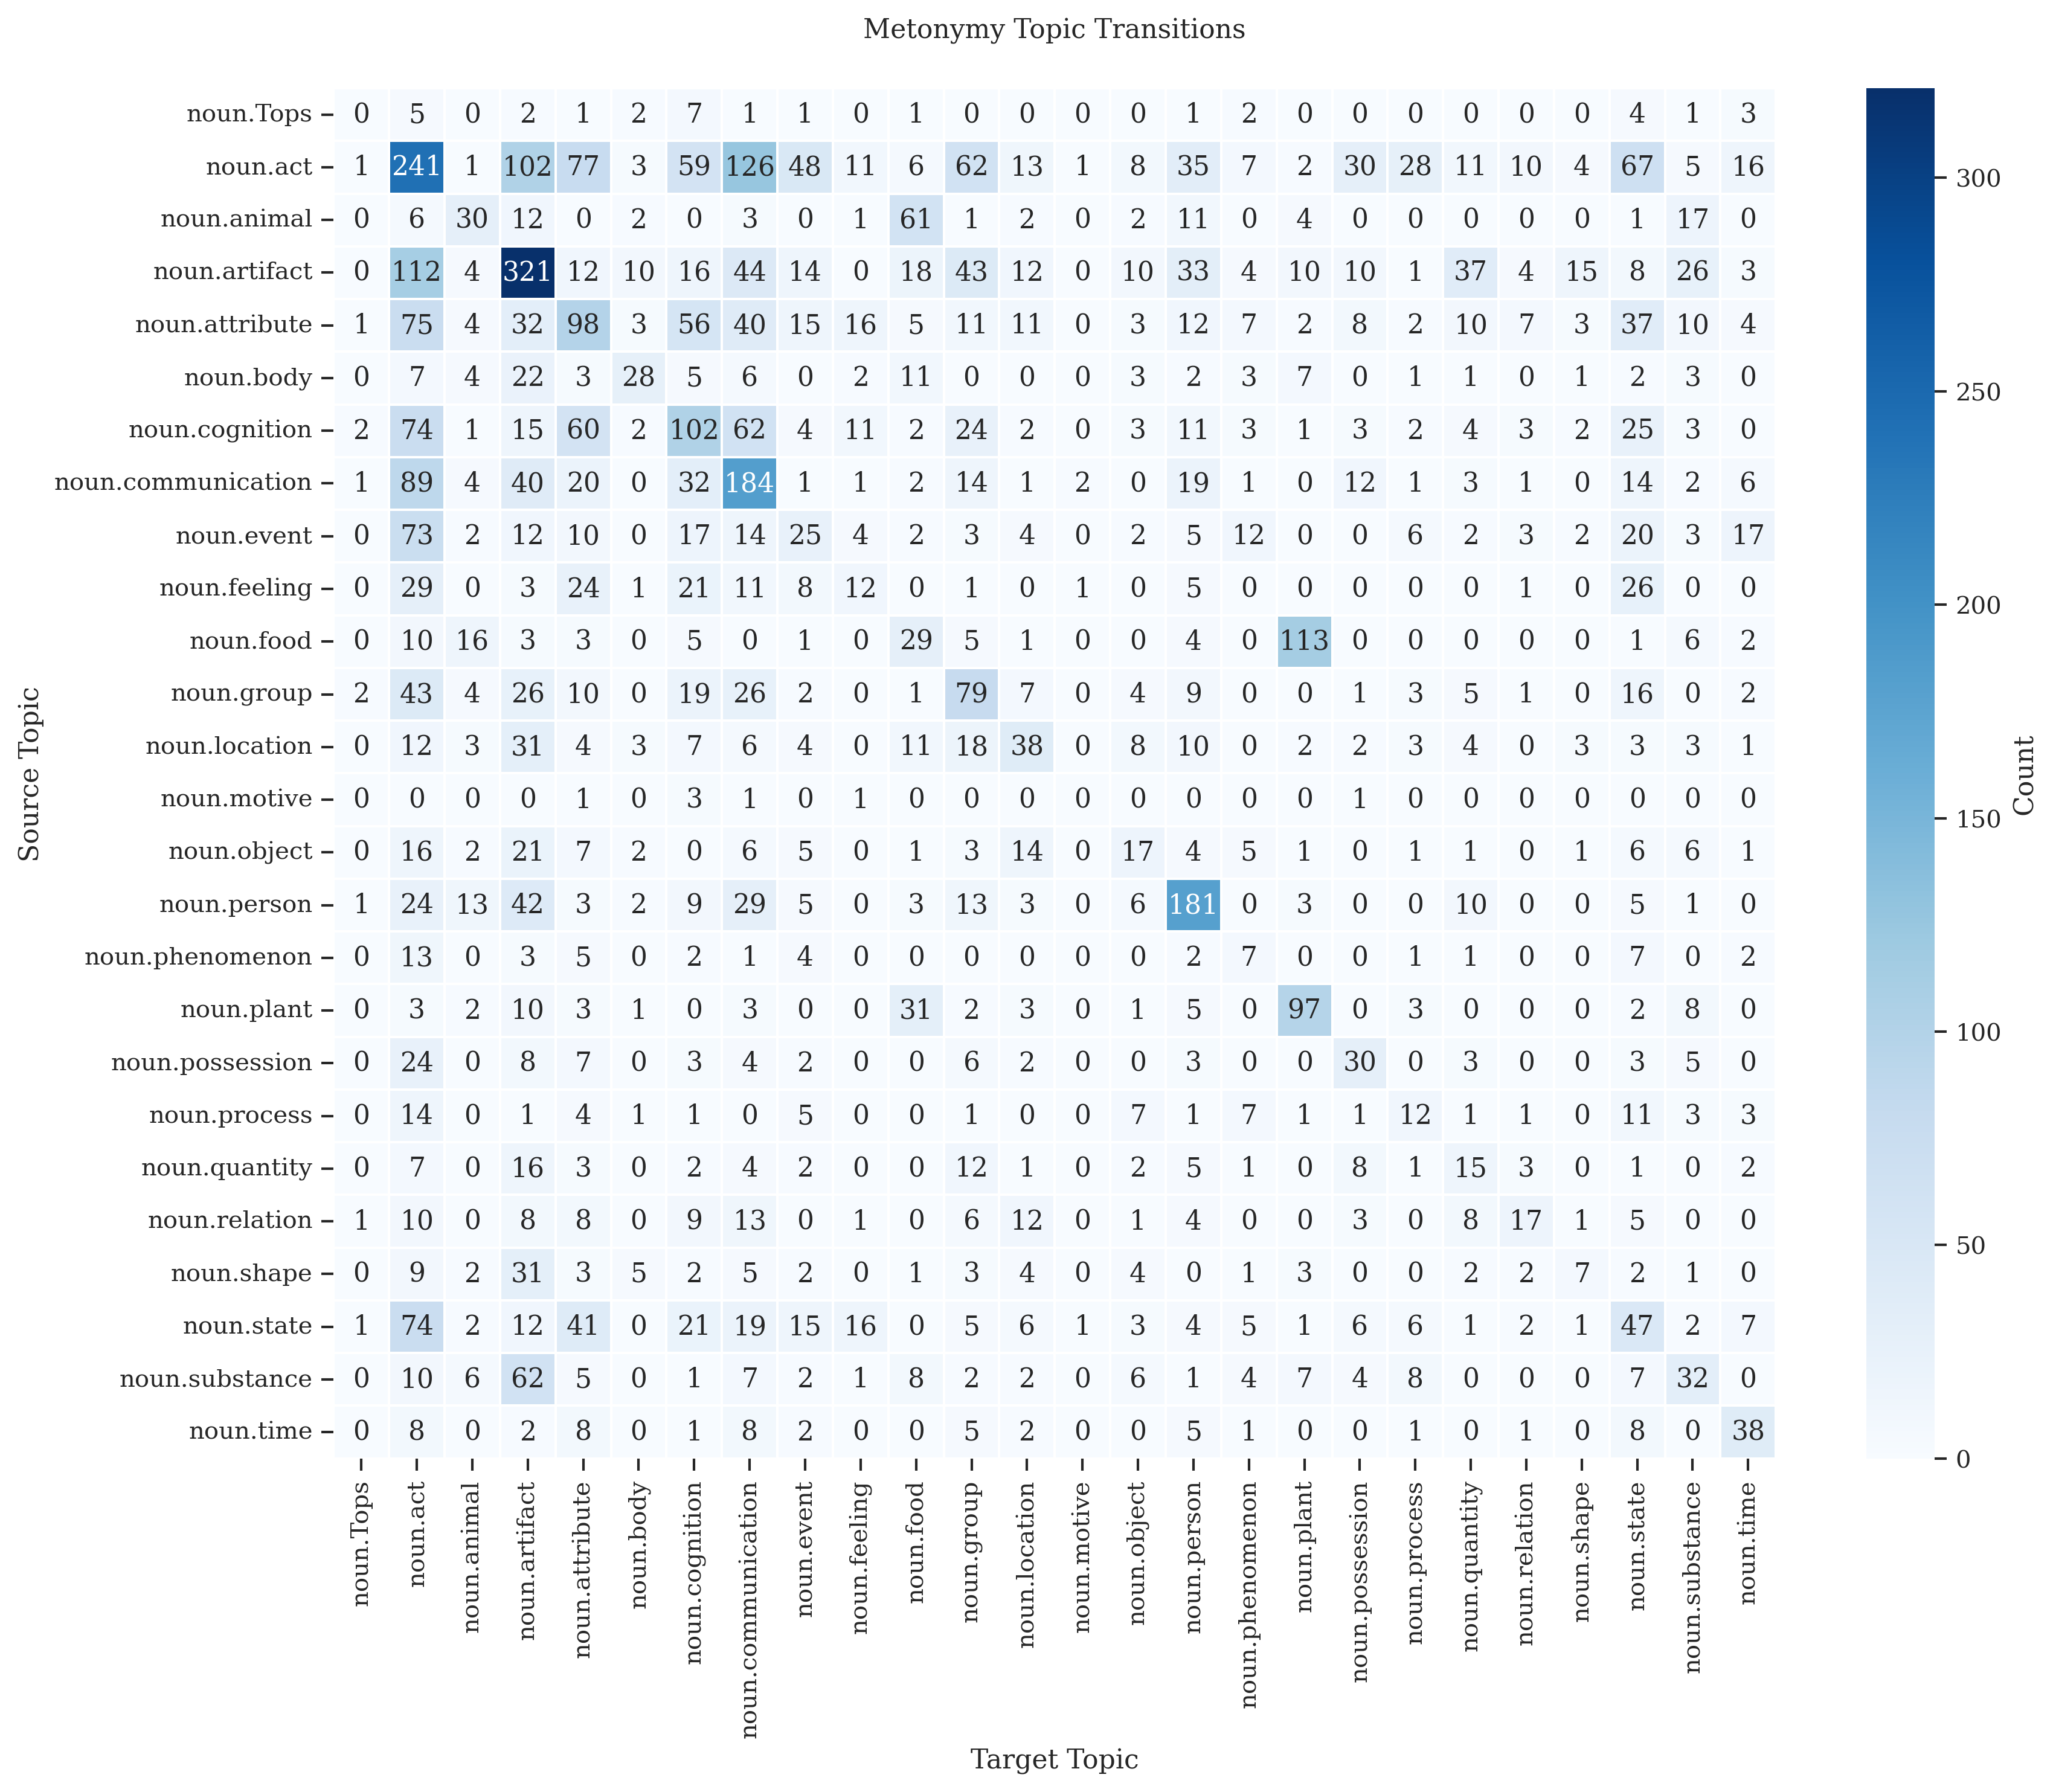
\includegraphics[height=0.9\textheight]{img/metonym_topic_heatmap.png}  
\end{frame}

\begin{frame}{We have only just begun}

Now investigating
  \begin{itemize}
\item Inclusiveness (Abstractness)
\item Frequency
\item Domain
\item Sentiment
\end{itemize}
\end{frame}
\section{Cross Lingual Exploration}
\begin{frame}{Can we see how English metaphors are used cross-lingually?}
  \begin{itemize}
  \item For example, are translations of linked pairs likely to be
    translated with the same word
    \begin{itemize}
    \item If so then metaphor/metonomy holds cross language
%    \item[\ldots] or this may indicate issues with automatic construction of wordnets
    \end{itemize}
  \item For example \eng{head} ``body part'' is metaphorically
    extended to ``person in charge'' in English and this is also true in Japanese,
    (\ja{頭}) Italian (\eng{capo}) and many other languages
  \item But not all metaphors are shared:  \eng{head} ``main part of a grammatical constituent'' is not \ja{頭} in Japanese
    \bigskip
  \item ChainNet is made for English, but we can expect many of the
    tropes to work with other languages
  \item If only we had a large collection of lexicons, linked by senses to English!
    

  \end{itemize}
\end{frame}

\subsection{The Open Multilingual Wordnet}
\begin{frame}
\frametitle{Introduction to Wordnets}

\begin{itemize}
    \item A wordnet is a lexical database that organizes words into sets of synonyms, called synsets.
    \item Each synset represents a unique concept,
      \\ capturing different senses of a word.
    \item Synsets are connected by semantic relations like hypernyms (superordinate) and hyponyms (subordinate).
    \item Wordnets are used in linguistic research, natural language processing (NLP), artificial intelligence, education and (a bit) language maintenance.
\end{itemize}
\end{frame}

\begin{frame}
\frametitle{History of Wordnets}

\begin{itemize}
\item Wordnet was first developed for English at Princeton University \citep{miller1995wordnet}.
  
    \item It was designed it as a model of human lexical memory.
    \item It became a foundational tool for computational linguistics and NLP.
    \item It has influenced the development of lexical resources for many other languages.
    \item Currently the Open English WordNet is maintained by John
      McCrae.  It is extending and revising the Princeton Wordnet.
\end{itemize}
\end{frame}


\begin{frame}{Many people wanted to have wordnets}

  \begin{itemize}
   \item \textbf{EuroWordNet} \citep{_Vossen:1998}:  
  Dutch, English, German, French, Spanish, Italian

  \item \textbf{BalkaNet}:  
  Bulgarian, Greek, Romanian, Serbian, Turkish

  \item \textbf{Asian WordNet}:  
  Japanese, Korean, Thai, Indonesian, Vietnamese, Mongolian, Burmese

  \item \textbf{IndoWordNet}:  
  Hindi, Bengali, Marathi, Gujarati, Punjabi, Urdu, Tamil, Telugu, Kannada, Malayalam, Odia, Assamese, Nepali, Konkani, Manipuri, Kashmiri, Sanskrit
\end{itemize}

And many individual projects not listed here.

\end{frame}

\begin{frame}{The synset for  \eng[tiger]{\ja{虎}}}
 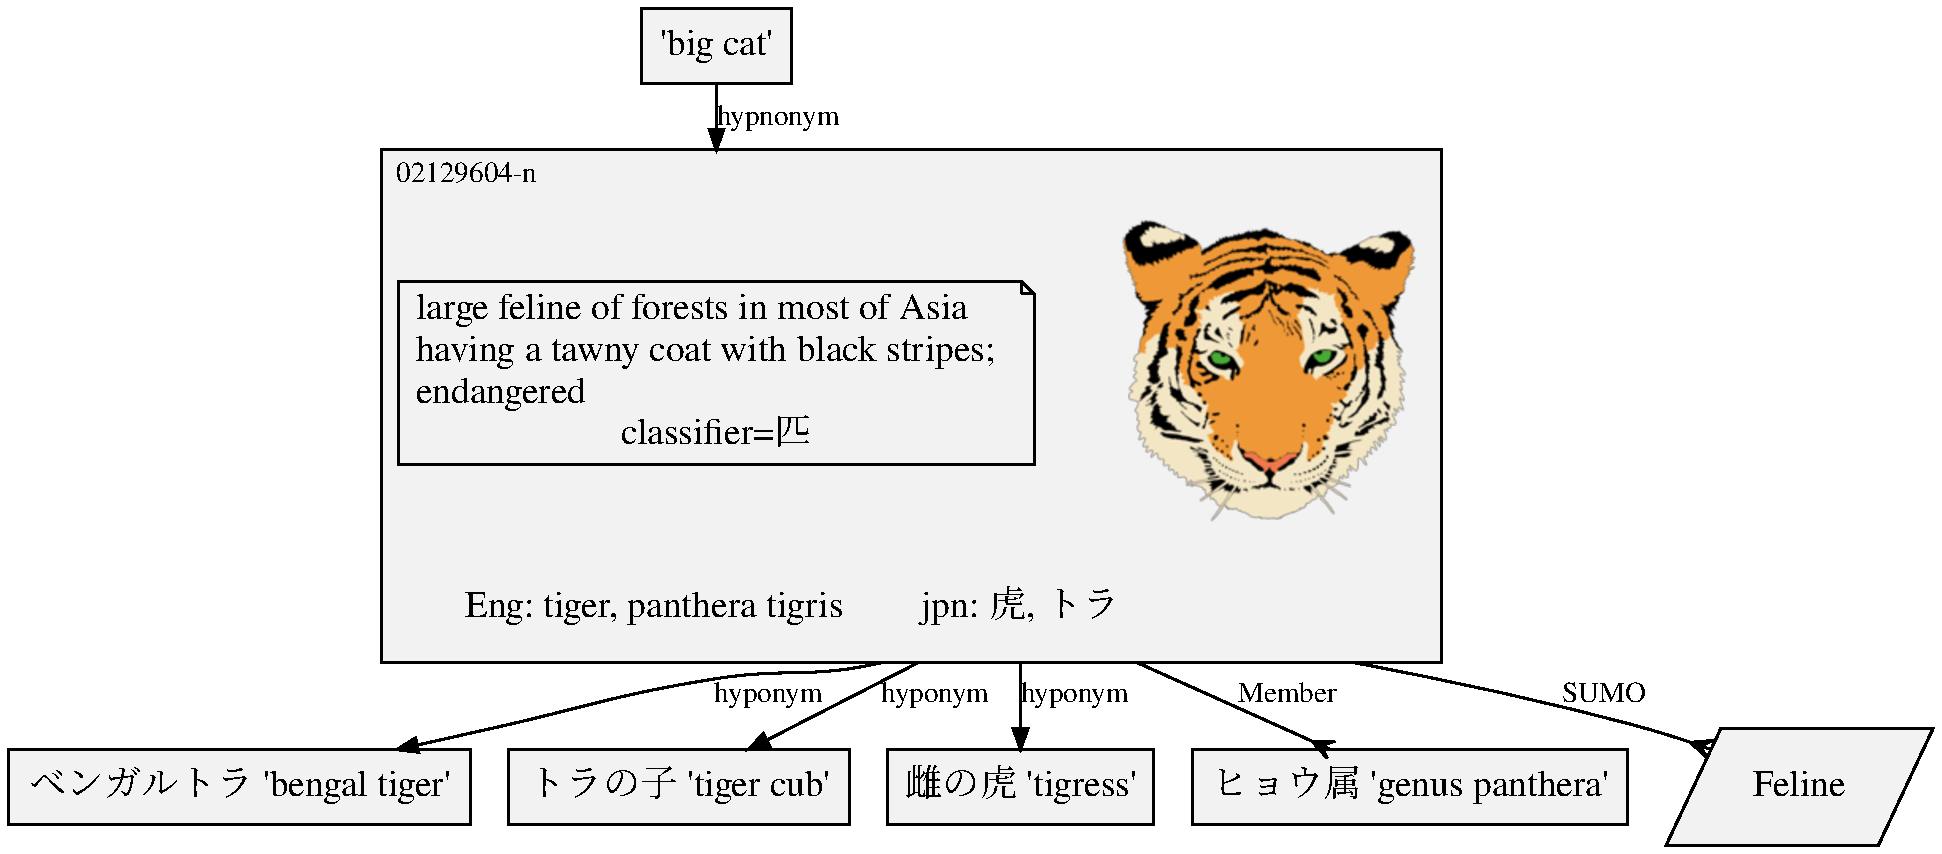
\includegraphics[width=0.9\textwidth]{img/wn-jpn-tiger.pdf}
\end{frame}


\begin{frame}
\frametitle{Multilingual Wordnets}

\begin{itemize}
    \item Over 50 hand built wordnets 
    \item Automatically-built Wordnets exist for over 1,200 languages \\ from Swadesh, Wiktionary and more
    \item Cross-lingual mappings help in tasks like machine translation and multilingual semantic analysis.
    \item The Open Multilingual Wordnet (OMW) provide free access to linked open wordnets.
\end{itemize}
\end{frame}

\begin{frame}
\frametitle{Challenges in Building Wordnets}

\begin{itemize}
    \item Developing wordnets requires careful analysis \\ impossible to automate
    \item Word meaning can be culturally specific, \\ requires careful consideration of local concepts.
    \item Data collection for under-resourced languages often involves fieldwork and expert collaboration.
    \item Validation and refinement of synsets is an ongoing process, especially for evolving languages.
    \item Many language resources are not open, so data cannot easily be shared.
\end{itemize}
\end{frame}

% \begin{frame}
% \frametitle{Building Wordnets for Under-resourced Languages}

% \begin{itemize}
%     \item Under-resourced languages may lack dictionaries, corpora, or standardized orthographies.
%     \item Wordnets for these languages require extensive collaboration with native speakers.
%     \item Data collection can involve workshops, interviews, and domain-specific lexicons.
%     \item Wordnet development can support language preservation and revitalization efforts.
%     \item These wordnets help document endangered languages and make them accessible for future research.
% \end{itemize}
% \end{frame}

\begin{frame}
\frametitle{Open Multilingual Wordnet (OMW)}

\begin{itemize}
    \item OMW is a free multilingual lexical database linking wordnets from many languages \citep{Bond:Foster:2013}
    \item OMW includes wordnets for widely spoken languages
    \item It also contains wordnets for under-resourced and endangered languages
    \item Researchers can access and contribute to OMW to support cross-linguistic studies
    \item The platform promotes collaborative development and data sharing across language communities
    \item In particular it has pushed open-licenses for the wordnets
\end{itemize}
\end{frame}

\begin{frame}{Wordnets in the world 2008}
\begin{center}
   \noindent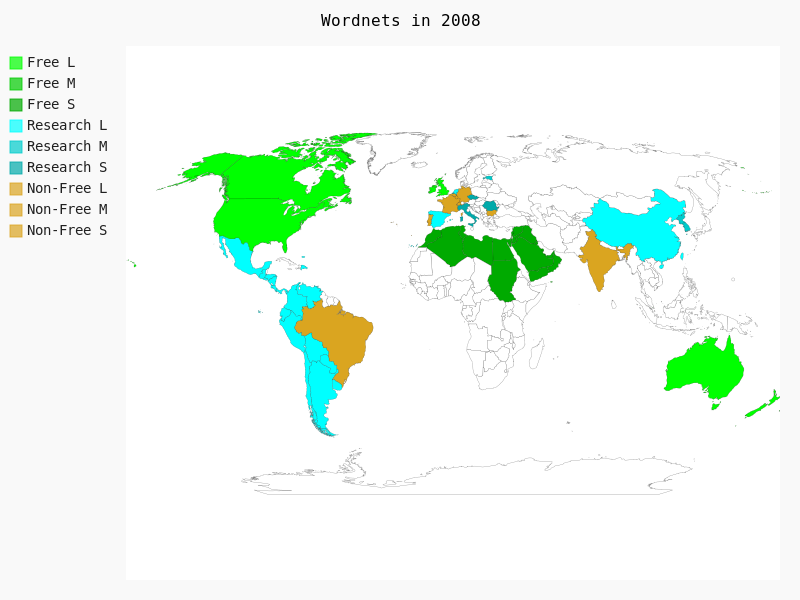
\includegraphics[width=1.0\textwidth]{img/wns-2008}
\end{center}
Green is free; Blue is research only; Brown costs money
\end{frame}

\begin{frame}{Wordnets in the world 2023}
\begin{center}
   \noindent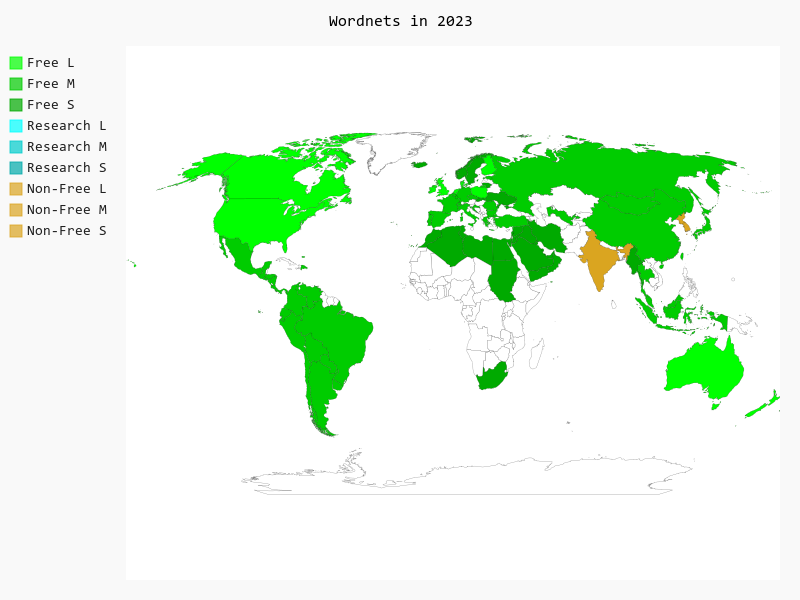
\includegraphics[width=1.0\textwidth]{img/wns-2023}
\end{center}
Green is free; Blue is research only; Brown costs money
\end{frame}

\begin{frame}{The situation is much better!  But not perfect}
  
\begin{itemize}
\item The map shows the situation only for the major language for each country
  \begin{itemize}
  \item India has over 450 living languages
  \item Indonesia has over 700 living languages
  \item Australia has over 100 indigenous languages and probably at least that many immigrant languages
  \item Even Czechia recognizes Belarusian, German, Polish, Hungarian, Ukrainian and  Vietnamese as official minority languages
  \end{itemize}
\item We are missing most of the world's languages
  \begin{itemize}
  \item Most wordnets start by exploiting existing resources
    \begin{itemize}
    \item  bootstrap off English
    \end{itemize}
  \item But most of the world's languages do not have lexicons linked
    to English!
  \end{itemize}
\end{itemize}

\end{frame}


% \begin{frame}
% \frametitle{Conclusion of the Introduction}

% \begin{itemize}
%     \item Wordnets are essential resources for understanding the semantic structure of languages.
%     \item They support a wide range of applications in NLP, linguistics, and AI.
%     \item Wordnets are now being developed for many languages, including those with limited resources.
%     \item Multilingual wordnets enable cross-linguistic research and better understanding of language relationships.
%     \item Wordnets contribute to preserving linguistic diversity by documenting and organizing lexical data.
% \end{itemize}
% \end{frame}


\begin{frame}{How are wordnets built?}

  \begin{itemize}
  \item Most new wordnets built be the \txx{expand} method --- the
    structure of Engish is used as a base, and new lemmas are added to the synsets
  \item Some wordnets are built by  the \txx{merge} method --- an existing lexical resources is merged with the English Wordnet
  \item The IndoWordnet \citep{Bhattacharyya:2010} used a clever hybrid
    \begin{itemize}
    \item a new structure was made for Hindi, using existing lexical resources 
    \item other Indic languages used this as a base for expand 
    \item but it is not under an open license, \ldots
    \end{itemize}

  \end{itemize}
  
So we have many lexicons, linked to English senses, of various sizes and qualities, built with different methods by different people, \ldots
  
\end{frame}





\begin{frame}{Measure the translation overlap with OMW}

  \begin{itemize}
  \item For every English word that has been annotated
    \begin{itemize}
    \item For each pair of English senses
    \item Look up all translations of each sense
      \\ measure the overlap (we use Jaccard similarity)
      \item Store and note if the senses are linked or not
    \end{itemize}
  \item So for example \eng{head} has 3 senses (really many more)
    \begin{enumerate}
    \item head, caput
      \\ \ja{ヘッド, \emp{頭}, 頭部}
    \item head, chief, top dog
      \\ \ja{大頭, 主任者, 御頭, 頭領, \emp{頭}}
    \item head,  head word
      \\ \ja{主要語}
    \end{enumerate}
  \item Overlap
    \begin{itemize}
    \item 1-2: 0.125 %(/ 1.0  8) 0.125
    \item 2-3: 0
    \item 1-3: 0
    \end{itemize}
  \end{itemize}
  

\end{frame}

\begin{frame}[allowframebreaks]{We do this for all the lexicons in OMW-1.4}

 
  \begin{center}
  \begin{tabular}{lrrrr}
    Lang & Unlinked & Metaphor & Metonomy & Non-Zero Instances \\ \hline
sv & 0.70 & 1.71 & 2.10 & 417   \\
he & 0.69 & 1.58 & 2.31 & 472   \\
eu & 0.82 & 1.30 & 1.80 & 5,562  \\
ja & 0.89 & 1.11 & 1.55 & 8,130 \\
ro & 0.83 & 1.30 & 1.71 & 6,429 \\
sq & 0.74 & 1.27 & 2.38 & 822 \\
%en & 0.97 & 1.08 & 1.07 & 33415 \\
da & 0.74 & 1.46 & 2.09 & 332 \\
lt & 0.63 & 1.46 & 2.86 & 692 \\
 \end{tabular}
\end{center}

\begin{itemize}
\item \txx{unlinked} has no link
\item \txx{metaphor} is linked by metaphor
\item \txx{metonymy} is linked by metonymy
\end{itemize}
Normalize by dividing  by the average distance for all senses.

  \begin{center}
  \begin{tabular}{lrrrr}
    Lang & Unlinked & Metaphor & Metonomy & Non-Zero Instances \\ \hline
es & 0.85 & 1.17 & 1.79 & 5,915 \\
 hr & 0.81 & 1.22 & 1.98 & 3,576 \\
    fr & 0.94 & 1.10 & 1.25 & 18,975 \\
nb & 0.73 & 1.49 & 2.12 & 339 \\
bg & 0.73 & 1.54 & 2.11 & 380 \\
gl & 0.70 & 2.13 & 1.55 & 271 \\
cmn & 0.74 & 1.57 & 1.97 & 1,347 \\
it & 0.80 & 1.39 & 1.81 & 4,614 \\
arb & 0.74 & 1.28 & 2.38 & 1,337 \\
pl & 0.75 & 1.43 & 2.07 & 1,326 \\
el & 0.72 & 1.30 & 2.45 & 1,274 \\
iwn & 0.79 & 1.46 & 1.80 & 968 \\
nn & 0.73 & 1.52 & 2.10 & 340 \\
id & 0.87 & 1.21 & 1.58 & 9,803 \\
  \end{tabular}
\end{center}

    \begin{center}
      \begin{tabular}{lrrrr}
    Lang & Unlinked & Metaphor & Metonomy & Non-Zero Instances \\ \hline
is & 0.73 & 1.51 & 2.13 & 388 \\
ca & 0.83 & 1.23 & 1.84 & 6,000 \\
sk & 0.73 & 1.35 & 2.31 & 2,067 \\
fi & 0.82 & 1.35 & 1.76 & 7,971 \\
nl & 0.79 & 1.38 & 1.90 & 2,991 \\
sl & 0.81 & 1.41 & 1.74 & 6,243 \\
th & 0.80 & 1.48 & 1.71 & 2,336 \\
pt & 0.80 & 1.26 & 1.96 & 5,414 \\
        zsm & 0.87 & 1.22 & 1.60 & 10,272 \\
        \midrule
Mean & 0.78 & 1.39 & 1.96 &  3,774\makebox[0mm]{~~~.3} 
  \end{tabular}
    \end{center}
    
  Unlinked  share fewer translations, metaphor shares more and metonomy shares much more.

  \Large Metonomy is more likely to hold cross linguistically!
  
\end{frame}

\begin{frame}{Discussion}

  \begin{itemize}
  \item The wordnets are of vastly different sizes: the number of sense
    pairs that have a translation varies from 271 (Galician) to 18,975 (French). 
  \item   Only Galician has the     score for metaphor (2.13) larger the score for metonymy (1.55), probably due to data sparsity. We would expect it to behave much like
    Portuguese (1.26/1.96).
  \item In order to measure perfectly how well tropes carry
    over between languages, we would need to mark metonymy and metaphor
    systematically for each language, and make sure all synsets for all
    senses have all relevant translations, \ldots 
  \item Without exception, senses linked by tropes are more likely to have an identical translation that those senses which are not linked
  \item With one exception, metonymy is more likely to have  an identical translation then metaphor  
  \end{itemize}

\end{frame}

\begin{frame}{Translations of the senses of \protect\eng{cherry}}
  \begin{center}
 \small 
  \begin{tabular}{llllll}% \toprule
    Sense & Mandarin & Japanese & Finnish & Italian & Portuguese \\ \midrule

    \sense{cherry}{1}   & \cn{樱桃木} & \ja{桜}, \ul{\ja{桜材}} & kirsikkapuumetsä & ciliegio  & cerejeira \\

    \sense{cherry}{2}  & \cn{樱桃树} & \ja{桜, 櫻} & kirsikkapuu & ciliegio  &  cerejeira\\

    \sense{cherry}{3}  & \cn{樱桃}  & \ja{桜桃, 桜ん坊} & kirsikka & cerasa , ciliegia  & ginja , cereja \\

    \sense{cherry}{4} &  \ul{\cn{樱桃红}} & \ul{\ja{桜ん坊色}}   &  kirsikanpunainen & ciliegia,  rosso ciliegia & cereja\ %\bottomrule
  \end{tabular}
\end{center}

\begin{itemize}
\item When we look at the translations, we see that the metonymy that is unmarked in English, is marked in other languages
\item Even within English, other synonyms have information
\end{itemize}

\end{frame}



\begin{frame}{Ongoing Research to Find Patterns}
  
\begin{itemize}
\item We can make a searchable database where the edges are decorated by the morphological differences
  \begin{itemize}
  \item So we can see all pairs linked by \dff{en:+ tree} or \dff{da:+træ} 
  \item The nodes link to synsets, so we can look
    up supertypes: we can say this link is of type  \lnk{food:plant}
  \\ or  \lnk{plant is food} in the cognitive linguistic style
  \item In this way we can group the tropes together in families
  \item Similar to \citet{Stoyanova:Mititelu:Leseva:Iordachioaia:2025}
  \end{itemize}
\item Other people have done this top down \cite[e.g start at \lnk{food:plant} and looked for examples]{khishigsuren_bella_brochhagen_marav_giunchiglia_batsuren_2022} 
\item With ChainNet we can go bottom-up and find many more patterns
  \begin{itemize}
  \item We can use multi-lingual features
  \item We need to investigate methods of clustering
  \item We need to find a good way of evaluating
  \end{itemize}
\item We would like to also map to existing Conceptual Metaphors
\end{itemize}

\end{frame}

\begin{frame}{The Patterns can be used Generatively}
  \begin{itemize}
  \item If we see a word that is of type \lnk{food}, then we can expect that
    there may be a kind of plant using the same word
    \begin{itemize}
    \item Useful for analyzing texts that otherwise don't make sense
    \item Can be used to analyse humour and word play \\
    \end{itemize}
  \end{itemize}

  \begin{center}
    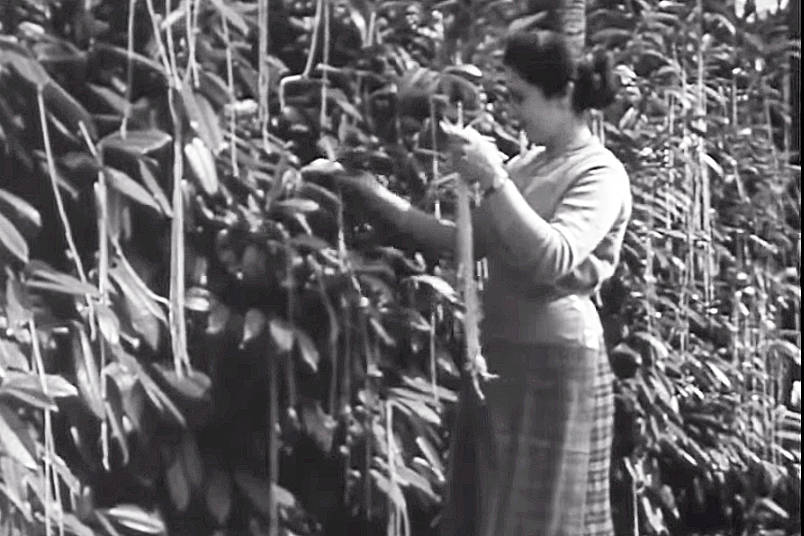
\includegraphics[width=0.5\textwidth]{img/spaghetti-tree.png} \\
    \href{https://en.wikipedia.org/wiki/Spaghetti-tree_hoax}{BBC Spaghetti Tree hoax (1957)}
  \end{center}
\end{frame}

\begin{frame}{We will mark metaphor/metonomy in more languages}
   \begin{tcolorbox}
   
\includegraphics{img/yami_cropped.png} \textit{yami}  \hfill (Japanese)\\ %闇 
   \wns{yami}{1} --- absence of light or illumination  \hfill (Japanese wordnet)\\
     \wns{yami}{2} --- an unilluminated area “he moved off into the darkness” \hfill (Japanese wordnet)\ \\
     \wns{yami}{3} --- absence of moral or spiritual values “the powers of darkness”  \hfill (Japanese wordnet)\\\
    \onew{\wns{yami}{4} --- an illegal market [\ldots ]} \hfill (not in English)
  \end{tcolorbox}
 \begin{tcolorbox}
     \wns{yami}{1} $\rightarrow$  \wns{yami}{2} (metonymy) \\
     \wns{yami}{1} $\rightarrow$  \wns{yami}{3} (metaphor) \\
     \wns{yami}{3} $\rightarrow$  \wns{yami}{4} (metaphor)
   \end{tcolorbox}
   We can start by projecting from English, then use the morphological patterns, \ldots
\end{frame}

\begin{frame}{Corpus-attested lexicalized metaphors for many languages: a range of views}

   
\includegraphics[width=0.5\textwidth]{img/bond_metaphor_plain.png} \hfill

   \begin{center}
        
\includegraphics[width=0.5\textwidth]{img/bond_metaphor_isl.png} \hfill
   \end{center}

 \hfill  
\includegraphics[width=0.5\textwidth]{img/bond_metaphor_desert.png}
% %  \caption{Corpus-attested lexicalized metaphors for many languages: a range of views}\label{fig:multi}
\end{frame}

 


  


\section{LLMs and Metaphors}


\begin{frame}{Metaphor in Large Language Models}
  \begin{itemize}
  \item Because these tropes are so established, LLMs capture the
    patterns well, and can generalise to novel examples, at least for languages with a lot of online data
  \item E.g. For Spanish, \citet{puraivan2024metaphor} found ChatGPT
    could differentiate literal from metaphorical senses with an
    accuracy of 85-88\% (on a small dataset)
    \begin{itemize}
    \item This is high enough to cause \txx{automation blindness}
    \item It is very hard for a human to spot mistakes
    \end{itemize}
  \item There are also interesting questions of how much metaphor
    interpretation in multilingual models is effected by other languages
    \\ The DanNet group have found metaphors in Danish not found in English are less likely to be recognized

  \end{itemize}%     

  
 \end{frame}

% --------------------------------------------------------
 \begin{frame}{Evaluating LLM-Generated Explanations of Metaphors
     \citep{Pedersen:Soerensen:Nimb:Hansen:Olsen:Al-Laith:2025} }

\begin{itemize}
  \item Metaphors have culturally distinct imagery and semantics (e.g., agricultural or national norms).
  \item Standard benchmarks (often English-centric) may hide biases against medium-resource languages.
  \item  LLMs may transfer English knowledge inappropriately to other languages.
\end{itemize}

\smallskip
\textbf{Models evaluated:}
\begin{itemize}
  \item \textbf{ChatGPT-4o mini} via web/API (multilingual, but English-heavy training)
  \item \textbf{Llama 3.1 405B}, large open model (multilingual but likewise English-biased).
\end{itemize}

\smallskip
Tested on a  culturally sensitive evaluation dataset of Danish metaphors \& model explanations.
\end{frame}

% --------------------------------------------------------
\begin{frame}{Dataset and Experimental Design}

  \textbf{Metaphor dataset:} 150 Danish expressions
  \begin{itemize}
  \item 75 single-word metaphors + 75 multiword idioms 
  \item Divided into:
    \begin{itemize}
    \item \textbf{Culture-specific} Danish metaphors (e.g., farming/nautical, social norms)
    \item \textbf{Cross-cultural} ones shared with English
    \end{itemize}
  \item Validated by native speakers and bilingual informants
  \end{itemize}

\medskip
\textbf{Prompting setup:}
\begin{itemize}
\item Four prompt variants:
  \begin{itemize}
  \item In isolation vs. with context
  \item Danish vs. English prompt language
  \end{itemize}
\item Each model generated 600 explanations (all combinations)
\end{itemize}

\medskip
\textbf{Evaluation:}
\begin{itemize}
  \item Human expert judges explanations on a 4-point qualitative scale
\end{itemize}

\end{frame}

% --------------------------------------------------------
\begin{frame}{Key Findings and Discussion}

\textbf{Main results:}
\begin{itemize}
  \item Both models explain \textbf{cross-cultural metaphors} far better than culture-specific ones
  \item Models show a strong \textbf{English bias} — higher quality explanations are produced when metaphors overlap with English
  \item Culture-specific sentiment and nuance are often lost in translation
\end{itemize}

\medskip
\textbf{Implications:}
\begin{itemize}
  \item Bias arises not only from data distribution but also from \emph{erroneous transfer} of English metaphorical knowledge. 
  \item Culturally grounded metaphor understanding in non-English languages remains a challenge for current multilingual LLMs
\end{itemize}

\end{frame}

% --------------------------------------------------------
\begin{frame}{Two examples}
  \begin{exe}
    \ex \eng{Han skød hendes argumenter ned.} \hfill Danish
    \trans He shot down her arguments.
  \end{exe}
  \begin{itemize}
  \item Correctly identifies metaphorical usage
  \item Maps \textbf{physical attack} $\rightarrow$ \textbf{argumentation}
  \item Produces fluent, accurate explanation
  \end{itemize}

  \begin{exe}
    \ex \eng{Han har rent mel i posen.} \hfill Danish
    \trans He has nothing to hide (Lit: He has clean flour in the bag.)
  \end{exe}
  \begin{itemize}
  \item Plausible but wrong English-based metaphor
    \\ “This metaphor refers to being prepared or well-supplied.”
  \item Over-literal explanation
    \\ “Clean flour symbolizes purity of intentions”
    but without connecting it to social trust / transparency
  \item Misses social–cultural grounding
  \end{itemize}

% LLMs handle metaphor well when it aligns with English conventions,  
% but struggle with \emph{lexicalized, culturally grounded metaphors}.

\end{frame}


\begin{frame}{Summary}
  
\begin{itemize}
\item The combination of detailed annotation of meaning (ChainNet \& Wordnet) and
  cross-lingual links (Open Multilingual) allow us to explore differences in lexicalized metaphor
  \begin{itemize}
  \item  Metonymy is based on association and contiguity
    \\ \txx{more universal} (average overlap 1.96 more than the baseline)
  \item  Metaphor often requires analogical reasoning and cultural framing
    \\ \txx{more culture and language specific} (average overlap 1.39 more than the baseline)
  \item Metaphor pairs are further apart that Metonym pairs
  \end{itemize}
\item We have shown these results hold over many languages
% \item We don't know if the tropes are independently discovered, come from a common ancestor, or are borrowed (the same problem as with cognates in etymology)

% \item LLMs may capture these regularities, but are hard to explore with
% \item Shared open lexicons allow us to look across languages
\end{itemize}

\end{frame}

\begin{frame}{Toward a broader understanding of Metaphor and Metonomy}
  \begin{itemize}
  \item Language is essential to our construction and transmission of knowledge
  \item Metaphors are the scaffolding for this construction
  \item For a full understanding of language we have to understand metaphors
  \item At the highest level, metaphors are very culturally embedded, to speak well you must understand the culture as well
    \begin{itemize}
    \item And the same language speakers will have many sub-cultures
    \end{itemize}
  \item Understanding cross-linguistic differences will help us understand cross-cultural differences
  \item Current metaphor research does not give us the comprehensive view we need to do this
    \begin{center}
      \large We are building an understanding based on a more complete view of language
    \end{center}
  \end{itemize}
\end{frame}


\section{Thanks}

\begin{frame}{Thanks and Resources}

  \begin{itemize}
  \item Thanks a lot to LOT for inviting me to present this work
  \item Thanks to all the many people who have worked on these
    resources, especially  Rowan Hall Maudslay, Luís Morgado da Costa and Joanna Ut-Seong Sio.
   \item Parts of this talk were presented at the Sprogteknologisk Konference 2024 and RegICON 2025
  \item If you are interested in wordnets or metaphor, come and talk to me!
  \end{itemize}
  \medskip
  \hrule
  \medskip
  \begin{itemize}
  \item ChainNet: \url{https://github.com/rowanhm/ChainNet}
    \begin{itemize}
    \item chainnet-xling: \url{https://github.com/bond-lab/chainnet-xling}
    \end{itemize}
  \item Open Multilingual Wordnet: \url{https:omwn.org}
  \end{itemize}

  
\end{frame}

\begin{frame}{We used these Wordnets}
  \begin{itemize}
  \item The combined wordnets include 
English \citep{_Fellbaum:1998}, 
Albanian \citep{Ruci:2008}, 
Arabic \citep{Black:Elkateb:Rodriguez:Alkhalifa:Vossen:Pease:Bertran:Fellbaum:2006}, 
Chinese \citep{Huang:Hsieh:Hong:Chen:Su:Chen:Huang:2010}, 
Danish \citep{Pedersen:2009}, 
Finnish \citep{Linden:Carlson:2010}, 
French \citep{Sagot:Fiser:2008}, 
Hebrew \citep{Ordan:Wintner:2007},
Indonesian and Malaysian (Nurril Hirfana et al., \citeyear{Noor:Sapuan:Bond:2011}), 
Italian \citep{Pianta:Bentivogli:Girardi:2002,Toral:Bracale:Monachini:Soria:2010}, 
Japanese \citep{Isahara:Bond:Uchimoto:Utiyama:Kanzaki:2008}, 
Norwegian Bokm\r{a}l and Norwegian Nynorsk (Lars Nygaard, personal communication 2012),
Persian \citep{Montazery:Faili:2010}, 
Portuguese \citep{Paiva:Rademaker:2012};
Polish \citep{Piasecki:Szpakowicz:Broda:2009}, 
Thai \citep{Thoongsup:Charoenporn:Robkop:Sinthurahat:Mokarat:Sornlertlamvanich:Isahara:2009},
and Basque, Catalan, Galician and Spanish \citep{Gonzalez-Agirre:Laparra:Rigau:2012}.
\item Data is available from \url{https://github.com/omwn/omw-data}
\item We used the python \defn{wn} module \citep{Goodman:Bond:2021}
\end{itemize}
\end{frame}

\begin{frame}[allowframebreaks]
        \frametitle{References}
        \bibliographystyle{aclnat}
        \bibliography{abb,mtg,ling,nlp}
\end{frame}


\end{document}

%%% Local Variables: 
%%% coding: utf-8
%%% mode: latex
%%% TeX-PDF-mode: t
%%% TeX-engine: xetex
%%% End: 
